\section{Informal development}
\label{sec:intuition}

Let us showcase all four new reasoning principles of \colosl by
sketching a proof of a simple, if slightly artificial example (we will
turn our attention to less contrived examples in
\S\ref{sec:examples}).

Consider the program $\mathbb{P}$ of \fig\ref{fig:concurrentInc},
written in pseudo-code, where variables $x$, $y$ and $z$ are allocated
on the heap and variable reading and mutation are understood as the
corresponding heap operations. After initialisation of the variables
to $0$, three threads are spawned to increment their values in
lock-step: $\mathbb{P}_x$ is the first allowed to run its increment
operation, then $\mathbb{P}_y$ and finally $\mathbb{P}_z$. This
process repeats until $x = y = z = 10$.

\begin{figure*}
\centering
\begin{tabular}{@{}l@{\ }|@{\ }l@{\ }|@{\ }l@{\ }|@{\ }l@{}}
  {$\mathbb{P}_x$:}& 
  {$\mathbb{P}_y$:}& 
  {$\mathbb{P}_z$:}&
  $\mathbb{P}$:\\[.5ex]
\begin{lstlisting}
//$\comment\{\shared{\cell{x}{0} * \cell{z}{0}}{I_x} * \token a_x\}$
while($x$ != 10)
//$\comment\left\{\shared{\begin{array}{@{}l<{\null}@{}l<{\null}@{}}\exsts{v}\cell{x}{v} * \cell{z}{v} \lor\\ \cell{x}{v+1} * \cell{z}{v}\end{array}}{I_x}\!\!\!\!\!\! * \token a_x\right\}$
{ $\langle$if ($x$ == $z$) $x$++;$\rangle$ }
//$\comment\left\{\shared{\begin{array}{@{}l<{\null}@{}l<{\null}@{}}\cell{x}{10} * \cell{z}{10} \lor\\ \cell{x}{10} * \cell{z}{9}\end{array}}{I_x}\!\!\!\!\!\! * \token a_x\right\}$
\end{lstlisting}
&
\begin{lstlisting}
//$\comment\left\{\shared{\begin{array}{@{}l<{\null}@{}l<{\null}@{}}\cell{x}{0} * \cell{y}{0} \lor\\ \cell{x}{1} * \cell{y}{0}\end{array}}{I_y}\!\!\!\!\!\! * \token a_y\right\}$
while($y$ != 10)
//$\comment\left\{\shared{\begin{array}{@{}l<{\null}@{}l<{\null}@{}}\exsts{v}\cell{x}{v} * \cell{y}{v} \lor\\ \cell{x}{v+1} * \cell{y}{v}\end{array}}{I_y}\!\!\!\!\!\! * \token a_y\right\}$
{ $\langle$if ($y$ < $x$) $y$++;$\rangle$ }
//$\comment\left\{\shared{\begin{array}{@{}l<{\null}@{}l<{\null}@{}}\cell{x}{10} * \cell{y}{10} \lor\\ \cell{x}{11} * \cell{y}{10}\end{array}}{I_y}\!\!\!\!\!\! * \token a_y\right\}$
\end{lstlisting}
&
\begin{lstlisting}
//$\comment\left\{\shared{\begin{array}{@{}l<{\null}@{}l<{\null}@{}}\cell{y}{0} * \cell{z}{0} \lor\\ \cell{y}{1} * \cell{z}{0}\end{array}}{I_z}\!\!\!\!\!\! * \token a_z\right\}$
while($y$ != 10)
//$\comment\left\{\shared{\begin{array}{@{}l<{\null}@{}l<{\null}@{}}\exsts{v}\cell{y}{v} * \cell{z}{v} \lor\\ \cell{y}{v+1} * \cell{z}{v}\end{array}}{I_z}\!\!\!\!\!\! * \token a_z\right\}$
{ $\langle$if ($z$ < $y$) $z$++;$\rangle$ }
//$\comment\left\{\shared{\begin{array}{@{}l<{\null}@{}l<{\null}@{}}\cell{y}{10} * \cell{z}{10} \lor\\ \cell{y}{11} * \cell{z}{10}\end{array}}{I_z}\!\!\!\!\!\! * \token a_z\right\}$
\end{lstlisting}
&
\begin{lstlisting}
//$\comment\{x|-> - * y|-> - * z|-> - \}$
$x$ = 0; $y$ = 0; $z$ = 0;
//$\comment\{x|-> 0 * y|-> 0 * z|-> 0 \}$
//$\comment\left\{\begin{array}{@{}l<{\null}@{}l<{\null}@{}}\shared{x|-> 0 * y|-> 0 * z|-> 0} I\\ \null*\token a_x * \token a_y * \token a_z\end{array}\right\}$
($\mathbb{P}_x$ || $\mathbb{P}_y$ || $\mathbb{P}_z$)
//$\comment\left\{\begin{array}{@{}l<{\null}@{}l<{\null}@{}}\shared{x|-> 10 * y|-> 10 * z|-> 10} I\\ \null*\token a_x * \token a_y * \token a_z\end{array}\right\}$
\end{lstlisting}
\end{tabular}

\begin{align*}
  I_x &\eqdef \left\{
  \begin{array}{@{}l@{}}
    \token a_x:\, \exsts{v} \cell{x}{v} * \cell{z}{v}  \swap  \cell{x}{v+1} * \cell{z}{v}\\
    \token a_z:\, \exsts{v} \cell{x}{v+1} * \cell{y}{v+1} * \cell{z}{v}\swap \cell{x}{v+1} * \cell{y}{v+1} * \cell{z}{v+1}
  \end{array}
  \right.\\
  I_y &\eqdef \left\{
  \begin{array}{@{}l@{}}
    \token a_x:\, \exsts{v} \cell{x}{v} * \cell{y}{v} * \cell{z}{v}  \swap  \cell{x}{v+1} * \cell{y}{v} * \cell{z}{v}\\
    \token a_y:\, \exsts{v} \cell{x}{v+1} *  \cell{y}{v}\swap \cell{x}{v+1} * \cell{y}{v+1}
  \end{array}
  \right.\\
  I_z &\eqdef \left\{
  \begin{array}{@{}l@{}}
    \token a_y:\, \exsts{v} \cell{x}{v+1} * \cell{y}{v} * \cell{z}{v}  \swap \cell{x}{v+1} * \cell{y}{v+1} * \cell{z}{v}\\
    \token a_z:\, \exsts{v} \cell{y}{v+1} *  \cell{z}{v}\swap \cell{y}{v+1} * \cell{z}{v+1}
  \end{array}
  \right.\\
  I &\eqdef \left\{
  \begin{array}{@{}l@{\,}l@{}r@{\ }c@{\ }l@{}}
    \token a_x: & \exsts{v} & \cell{x}{v} * \cell{z}{v} & \swap & \cell{x}{v+1} * \cell{z}{v}\\
    \token a_y: & \exsts{v} & \cell{x}{v+1} * \cell{y}{v} & \swap & \cell{x}{v+1} * \cell{y}{v+1}\\
    \token a_z: & \exsts{v} & \cell{y}{v+1} * \cell{z}{v} & \swap & \cell{y}{v+1} * \cell{z}{v+1}
  \end{array}\right.
\end{align*}

\hrule\vspace{5pt}
\caption{The concurrent increment program together with a \colosl proof
  sketch. Lines starting with \lstinline{//} contain formulas that describe
  the local and subjective shared state at relevant program point.}
\label{fig:concurrentInc}
\end{figure*}

\subsection{\colosl assertions}
\label{subsec:intuition}

In this proof sketch, we use \colosl assertions to describe program
states. As will be formalised in \S\ref{sec:logic}, we extend
\emph{separation logic} assertions~\cite{rey02} with subjective views,
and interpret \colosl assertions over a particular domain that
includes a \emph{local} state, a \emph{subjective} state, and
interference \emph{actions}. These instrumented states are linked to
machine states in our soundness proof based on Views and presented in
\S\ref{sec:soundness}. A pointsto predicate $x |-> y$ denotes those
states whose local heap is the singleton heap where the only allocated
address is $x$, and it points to value $y$. An assertion $P_1 * P_2$
splits the local state into two \emph{disjoint} heaps and the
subjective state into two \emph{overlapping} heaps such that the
corresponding substates satisfy $P_1$ and $P_2$, respectively. A
\emph{subjective view} $\shared{P}{I}$ is true if the subjective state
satisfies $P$ and is subject to interferences in $I$.

\begin{figure}
\centering
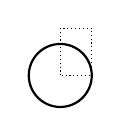
\begin{tikzpicture}
\draw[thick] (0,0) circle (.4cm);
\draw[densely dotted] (0,0) rectangle (.4cm,.6cm);
\end{tikzpicture}
\quad$\swap$\quad
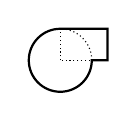
\begin{tikzpicture}
\draw[densely dotted] (0,0) circle (.4cm);
\draw[densely dotted] (0,0) rectangle (.6cm,.4cm);
\draw[thick] (.4cm,0) arc (0:-270:.4cm) -- (.6cm,.4cm) -- (.6cm,0) -- cycle;
\end{tikzpicture}\\


\null\hfill

\begin{tikzpicture}[baseline,yshift=.1cm]
\draw[thick] (0,0) circle (.4cm);
\end{tikzpicture}\quad subjective state
\hfill
$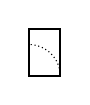
\begin{tikzpicture}[baseline,yshift=-.25cm]
\draw[thick] (0,0) rectangle (.4cm,.6cm);
\draw[densely dotted] (.4cm,0) arc (0:90:.4cm);
\end{tikzpicture}|= P$
\hfill
$
\begin{tikzpicture}[baseline]
\draw[thick,yshift=-.1cm] (0,0) rectangle (.6cm,.4cm);
\end{tikzpicture}|= Q$
\hfill\null

\vspace{5pt}\hrule\vspace{5pt}
\caption{Effect of an action $P\swap Q$.}
\label{fig:action}
\end{figure}

Interferences in $I$ are of the form $\token{a}: P \swap Q$ where
$\token{a}$ denotes a \emph{capability} associated with \emph{action}
$P \swap Q$. $P$ represents the action pre-condition and describes the
part of the shared state required to carry out the action, while $Q$
is the action post-condition and describes the part of the shared
state after the action.  A thread in possession of a given capability
in its local state can perform the associated action and update the
shared state accordingly provided that the contents of the shared
state satisfy the action pre-condition.  For instance, as the name
suggests, the action associated with capability $\token a_x$ in $I_y$,
corresponds to the update of variable $x$: for any $v$, if
$\cell{x}{v} * \cell{y}{v} * \cell{z}{v}$, a thread in possession of
$\token a_x$ in its local state can increment $x$.  A particularity of
\colosl is that actions can be performed by the environment any time
their precondition is \emph{compatible} with the current subjective
state, as represented schematically in \fig\ref{fig:action}, and not
only when the precondition is satisfied by a \emph{substate} of the
subjective state (as is required for the program to perform the
action). In particular, an action whose precondition is satisfiable is
\emph{always} enabled from the empty subjective view (which by
definition is compatible with all other states).

Assertions appearing in pre and postconditions of triples must be
\emph{stable}. That is, for any action permitted by $I$, where $I$ is
the interference relation of a subjective view appearing in the
assertion, if the current thread does not exclusively hold the
associated capability (and thus the action may be performed by the
environment at any time), the assertion must remain true after the
action has taken place (see \fig\ref{fig:action}). For instance, the
assertion
\[
\token a_x * \token a_y * \shared{x|->0 * y|->0}{I_y}
\]
is stable since it owns the capabilities associated with both actions
of $I_y$ ($\token a_x$ and $\token a_y$), hence no other thread can
perform an action that would invalidate $x|->0 * y|->0$. On the other
hand, the assertion
\[
\token a_y * \shared{x|->0 * y|->0}{I_y}
\]
is not stable since a thread in possession of $\token a_x$ can
potentially increment the value of $x$ and thus invalidate $x|->0 *
y|->0$.

%%%%%%%%%%%%%%%%%%%%%%%%%%%%%%%%%%%%%%%%%%
\subsection{Extending the shared region}
\label{subsec:extend}

The program state in \colosl is modelled by two components
representing a thread-local (private) state exclusively visible to the
thread, and a shared state accessible by all threads. At the very
beginning of the execution of $\mathbb{P}$, the state is purely local
and contains the three variables $x$, $y$, and $z$, which allows
$\mathbb P$ to initialise them to 0. Since the purpose of the rest of
the program is to share these variables between $\mathbb P_x$,
$\mathbb P_y$, and $\mathbb P_z$, a shared region is created, ruled by
interferences $I$ and the three tokens $\token a_x$, $\token a_y$, and
$\token a_z$. The capabilities are automatically added to the current
local state upon region creation:
\begin{align}
  \label{eq:extend}
  P \containI I
  &\text{ implies }
  P \Vvdash
  \exsts{\capAss{1}, \capAss{2}} \capAss{1} * \shared{P *
    \capAss{2}}{I}
  \tag{\textsc{Extend}}
\end{align}
A relation $P\Vvdash P'$ means that it is safe to substitute $P$ for
$P'$ (resp.\ $P'$ for $P$) in the precondition (resp.\ postcondition)
of any triple (hence if $P|- P'$ then $P\Vvdash P'$).
\julescomment{TODO: say more about $\Vvdash$, perhaps a reference?}
The existential quantification of capabilities is to ensure the
\emph{freshness} of the generated capabilities. The side condition $P
\containI I$ ensures that the mutations performed by actions in $I$
are confined to $P$, hence do not contradict existing views of the
shared state. This notion will be formalised in
\S\ref{subsec:extension}.


%%%%%%%%%%%%%%%%%%%%%%%%%%%%%%%%%%%%%%%%%
\subsection{Combining Subjective Views}
\label{subsec:merge}

The next step is to distribute the state to the three threads. This is
done, as is standard in variants of separation logic, using the
following concurrency rule:
\[
\infrule{Parallel}
        {\hoare{P_1}{\mathbb{P}_1}{Q_1}\\
          \hoare{P_2}{\mathbb{P}_2}{Q_2}}
        {\hoare{P_1 * P_2}{\mathbb{P}_1 || \mathbb{P}_2}{Q_1 * Q_2}}
        {}
\]



The capabilities $\token a_x$, $\token a_y$ and $\token a_z$ are
passed to $\mathbb P_x$, $\mathbb P_y$ and $\mathbb P_z$. The
subjective shared state is split using $*$ and the following principle
of \colosl:
\begin{align*}
  \shared{P}{I_1} * \shared{Q}{I_2} &\vdash \shared{P \sepish Q}{I_1 \cup I_2} \tag{\textsc{Merge}}
\end{align*}
Since a shared state assertion $\shared{P}{I}$ defines contents of
parts of the shared state, multiple threads can view different,
potentially overlapping parts of the shared state. As such, the
separating conjunction $*$ behaves as \emph{overlapping conjunction}
$\sepish$~\cite{rey-slnotes,ramification} (sometimes called
\emph{sepish}~\cite{gareth-js12}).

Consequently, as in the case of the first and second lines of the
above derivation $\shared{P_0}{I} * \shared{P_0}{I} \iff
\shared{P_0}{I}$. Upon dividing the capabilities between the three
threads, the $\shared{P_0}{I}$ assertion is no longer stable and is
thus weakened into the stable assertion $G$. Predicate $G$ describes
the contents of the shared state as three disjuncts corresponding to
various points in execution of $\mathbb{P}$.


In order to establish the desired post-condition, at this stage we
need to \emph{merge} the subjective views of all three threads and
obtain a stronger view such as that of $G'$ in
\fig\ref{fig:concurrentIncCoLoSLSpec}.
\begin{align*}
  \label{eq:merge}
  \shared{P}{I_1} * \shared{Q}{I_2} &\vdash \shared{P \sepish Q}{I_1 \cup I_2} \tag{\textsc{Merge}}
\end{align*}
By two applications of the \textsc{Merge} rule, we can merge $S'_x$,
$S'_y$ and $S'_z$ and obtain $\shared{\cell{x}{10} * \cell{y}{10} *
  \cell{z}{10}}{I_x \cup I_y \cup I_z}$. Finally, through an
application of \textsc{Shift} rule, we can rewrite $I_x \cup I_y \cup
I_z$ into $I$ as specified in \fig\ref{fig:concurrentIncCoLoSLSpec}
and obtain $G'$.



%%%%%%%%%%%%%%%%%%%%%%%%%%%%%%%%%%%%%%
\subsection{Forgetting shared state}
\label{subsec:hide}

We are now left with justifying the proofs of each individual thread,
made in isolation.

Note that thread $\tau_x$ is only concerned with the values of $x$ and
$z$; \emph{mutatis mutandis} for $\tau_y$ and $\tau_z$. However, with
the specification of \fig\ref{fig:concurrentIncCoLoSLSpec}, all three
variables are visible by $\tau_x$ and as such in verification of
$\mathbb{P}_x$ it is necessary to account for the interference
associated with $y$ even though its value is neither read nor modified
by $\tau_x$. In other words, the specification of
\fig\ref{fig:concurrentIncCoLoSLSpec} is not \emph{local}
enough. Ideally, $\tau_x$'s view of the shared state would be of the form $\shared{P_x}{I}$ with predicate $P_x$ as defined below where variable $y$ is \emph{forgotten}.
\[
	P_x \eqdef \exsts{v} \cell{x}{v} * \cell{z}{v} \lor \cell{x}{v+1} * \cell{z}{v}
\]
In \colosl\ it is always possible to forget parts of the shared state
and arrive at a \emph{subjective}, more local and thus weaker view of
the shared state. That is\footnote{Since $P ** Q |- P * \m{true}$, we
  have $\shared{P ** Q}{I} \vdash \shared{P}{I}$ by~\eqref{eq:forget}.},
\begin{align*}
  \label{eq:forget}
  \shared{P * Q}{I} &\vdash \shared{P}{I}  \tag{\textsc{Forget}}
\end{align*}
%where $P \sepish Q$ denotes the \emph{overlapping conjunction} or ``sepish'' \cite{}\footnote{Since $P * Q \vdash P \sepish Q$, from the \textsc{Hide} rule we have $\shared{P * Q}{I} \vdash \shared{P}{I}$}. 
However, the right-hand-side is not necessarily stable with respect to $I$. For instance, in the case of $\shared{P_x}{I}$ above where $I$ is as specified in \fig\ref{fig:concurrentIncCoLoSLSpec}, since we no longer know the value of $y$ in relation to $x$ and $z$, the action associated with capability $\token a_z$ can be carried out by the environment and change the value of $z$. As such, the strongest stable assertion we can derive is: 
\[
	\shared{\exsts{v, v'}  \cell{x}{v} * \cell{z}{v'}}{I}
\]


%%%%%%%%%%%%%%%%%%%%%%%%%%%%%%
\subsection{Action Shifting}
\label{subsec:shift}

In the case of the less local predicate $G$, whenever the
pre-condition of the action associated with $\token a_z$ is satisfied
(third disjunct), it is also the case that $\cell{x}{v+1}$. In other
words, in all the cases where the shared state satisfies
$\cell{y}{v+1} * \cell{z}{v}$, it also satisfies $\cell{x}{v+1} *
\cell{y}{v+1} * \cell{z}{v}$. However, this information is not
reflected in $I$ and as a result when weakening $G$, we need to
stabilise the resultant assertion which proves to be very weak. To
remedy this, in \colosl we introduce the notion of action
\emph{shifting} (rewriting) with respect to the \emph{invariant} of
the shared state. Given $\shared{P}{I'}$, we write $\fence{} \fences
(P, I')$ - read ``$\fence{}$ fences $P$ with respect to $I'$'' - to
indicate that i) $\fence{}$ contains all states associated with $P$
and ii) it is closed under $I'$; that is, given any action in $I'$
whose pre-condition is satisfied by a state in $\fence{}$, the state
resulting from the action is also in $\fence{}$. For instance, given
the $G$ predicate of \fig\ref{fig:concurrentIncCoLoSLSpec}, we have
$\fence{G} \fences (P_G, I)$ where $P_G$ denotes the assertion inside
the box and $\fence{G}$ is as specified below.
\[
	\begin{array}{l l}
		\fence{G} = \hspace*{-5pt}& \left\{\cell{x}{v} * \cell{y}{v} * \cell{z}{v} ||| v \in \{0, \cdots 10\} \right\} \\
		& \cup \left\{\cell{x}{v+1} * \cell{y}{v} * \cell{z}{v} ||| v \in \{0, \cdots 9 \} \right\} \\
		& \cup \left\{\cell{x}{v+1} * \cell{y}{v+1} * \cell{z}{v} ||| v \in \{0, \cdots 9\} \right\}\\
	\end{array}
\]
%as well as the action associated with its update
Given the above invariant, we can now \emph{shift} the action associated with $\token a_z$ in $I$ and arrive at $I'$ where
\[
	I' \eqdef \left\{
		\begin{array}{@{}l@{}}
			\token a_x:\, \exsts{v} \cell{x}{v} * \cell{z}{v}  \swap  \cell{x}{v+1} * \cell{z}{v}\\
			\token a_y:\, \exsts{v} \cell{x}{v+1} * \cell{y}{v}  \swap  \cell{x}{v+1} * \cell{y}{v+1}\\
			\token a_z:\, \exsts{v} \cell{x}{v+1} *
                        \cell{y}{v+1} * \cell{z}{v} \swap\null\\
			\hspace*{2cm} \cell{x}{v+1} * \cell{y}{v+1} * \cell{z}{v+1}\\
		\end{array}			
	\right.
\]
Note that in doing so we have neither restricted nor relaxed the action of $\token a_z$ in that it can be carried out in exactly the same states given the invariant $\fence{G}$. This is formalised by the \textsc{(Shift)} rule where $I \weakenI{\fence{}} I'$ denotes the shifting of $I$ with respect to $\fence{}$ and we defer its formalisation to \S\ref{sec:logic}.
\[
	\text{if}\hspace*{0.25cm} \fence{} \fences (P, I) 
	\hspace*{0.25cm}\text{and}\hspace*{0.25cm} I \weakenI{\fence{}} I'
	\hspace*{0.25cm}\text{then}\hspace*{0.25cm}
	\shared{P}{I} \Vvdash \shared{P}{I'} \hspace*{0.5cm} \textsc{(Shift)}
\]
Given predicate $G$ of \fig\ref{fig:concurrentIncCoLoSLSpec}, we can first shift $I$ into $I'$ (specified above) using the \textsc{Shift} rule and then apply the \textsc{Forget} rule to forget variable $y$ and obtain $\shared{a_x}{I'}$.
%%
%\[
%	X' \eqdef \shared{\exsts{v} \cell{x}{v} * \cell{z}{v} \lor \cell{x}{v+1} * \cell{z}{v}}{I'} 
%\]
%%
We have almost arrived at a local specification for $\mathbb{P}_x$. However, the action of $\token a_y$ is still visible in $I'$ even though it does not affect the values of $x$ or $z$. Through interference shifting, we can not only rewrite actions with respect to the invariant, we can also \emph{forget} actions that affect \emph{none} of the states contained in the invariant. For instance, let $\fence{x} = \left\{\cell{x}{v} * \cell{z}{v} ||| v \in \{0, \cdots 10\} \right\} \cup \left\{\cell{x}{v+1} * \cell{z}{v} ||| v \in \{0, \cdots 9 \} \right\}$, then we have $\fence{X} \fences (X, I')$. In the case of the action of $\token a_y$, given any state $p$ in the action pre-condition (e.g. $p = \cell{x}{1} * \cell{y}{0}$), for an arbitrary state $s \in \fence{X}$ (e.g. $s = \cell{x}{1} * \cell{z}{0}$), \emph{all overlaps} of $p$ and $s$ ($p \meetL s = \{\cell{x}{1}\}$) are preserved by the action. We give the formal definition of overlap operator $\meetL$ in \S\ref{sec:logic}. 

Given $I'$ and $\fence{X}$ we can again apply the \textsc{Shift} rule in order to forget about the action of $\token a_y$ and obtain $I_x$ as specified in \fig\ref{fig:concurrentIncSubjectiveSpec}. We can take analogous steps in order to obtain subjective views $S_y$ and $S_z$ for threads $\tau_y$ and $\tau_z$. We then pass the $\token a_x$, $\token a_y$ and $\token a_z$ capabilities to $\tau_x$, $\tau_y$ and $\tau_z$ and verify $\mathbb{P}$ as follows:
\[
\hspace*{-0.2cm}
\begin{array}{c}
	\color{blue}{\left\{\token a_x * \token a_y *  \token a_z *  S_x * S_y * S_z \right\}}\vspace*{2pt}\\
	
	\begin{array}{c || c || c}
		\color{blue}{\left\{\token a_x * S_x \right\}} & \color{blue}{\left\{\token a_y * S_y \right\}} & \color{blue}{\left\{\token a_z * S_z \right\}}\\
		&&\vspace*{-7pt}\\
		\mathbb{P}_x & \mathbb{P}_y & \mathbb{P}_z\\
		&&\vspace*{-5pt}\\

		\color{blue}{
			\left\{
					\token a_x * S'_x
			\right\}
		} 
		& 
		\color{blue}{
			\left\{
				\token a_y * S'_y
			\right\}
		} 

		&
		
		\color{blue}{
			\left\{
				\token a_z * S'_z
			\right\}
		} 		
		\vspace*{3pt}
	\end{array}\\
	\color{blue}{\left\{\token a_x * \token a_y *  \token a_z *  S'_x * S'_y * S'_z \right\}}\\
\end{array}
\]
with
\[
\begin{array}{l l}
	S'_x \eqdef & \shared{\cell{x}{10} * \cell{z}{10} \lor \cell{x}{10} * \cell{z}{9} }{I_x}\\
	S'_y \eqdef & \shared{\cell{x}{11} * \cell{y}{10} \lor \cell{x}{10} * \cell{y}{10} }{I_y}\\
	S'_z \eqdef & \shared{\cell{y}{11} * \cell{z}{10} \lor \cell{y}{10} * \cell{z}{10} }{I_z}
\end{array}
\]
